\documentclass[aps,prl,reprint,amsmath,amssymb]{revtex4-2}
\usepackage{graphicx}
\begin{document}
\title{Synthetic two-mode response: a single- and double-column layout demonstration}
\author{Illustrative example only}
\affiliation{No experimental result or publication claim}
\begin{abstract}
This deliberately short synthetic example demonstrates a title and abstract, a single-column pole plot, and a double-column response map. Its linear model is exactly specified; its floats illustrate REVTeX behavior rather than a recommended figure count or a complete manuscript. The model connects a slowly decaying normal mode to delayed transfer when the coupling is below the pole-coalescence threshold.
\end{abstract}
\maketitle
\raggedbottom
\setlength{\parskip}{0pt}
\textit{Physical question.---}A narrow spectral structure need not by itself identify where an excitation is stored. Frequency-domain response and time-domain evolution probe related aspects of a coupled system, but a proposed explanation must also respect the actual eigenvalues. This example uses two linearly coupled damped modes to make those distinctions explicit. It contains no claim of novelty and no fabricated bibliography.

\textit{Model.---}Let the amplitude generator be
\begin{equation}
A=\begin{pmatrix}-\kappa_a/2-i\Delta&-ig\\-ig&-\kappa_b/2\end{pmatrix},
\end{equation}
with $\kappa_a=1$ and $\kappa_b=0.08$. At $\Delta=0$, the eigenvalues are $-0.27\pm\sqrt{0.23^2-g^2}$. Thus $g=0.1$ has distinct fast and slow decay rates, whereas $g=0.25$ has two eigenvalues with equal real part. The pole trajectory in Fig.~\ref{fig:poles} displays this distinction directly. A slow-pole explanation cannot be carried unchanged across that threshold.
\begin{figure}[tb]
\centering
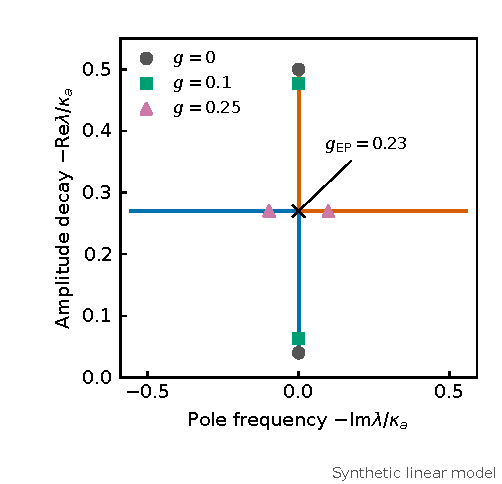
\includegraphics[width=\columnwidth]{../mechanism-examples/pole_trajectory.pdf}
\caption{Synthetic model pole trajectory. The supplied script computes the eigenvalues; the figure is placed in a single-column float. Its exact eventual position is chosen by REVTeX.}
\label{fig:poles}
\end{figure}

\textit{Discriminating evidence.---}For a drive on mode $a$, the frequency response follows from the inverse of $-i\omega I-A$. Figure~\ref{fig:response} combines a detuning-frequency map with a representative spectral cut. The wide format provides room for complementary evidence; it is not required merely because the target is PRL. Coupling, loss, detuning and frequency have explicitly defined roles, and the calculation does not supply measurement uncertainties.
\begin{figure*}[t]
\centering
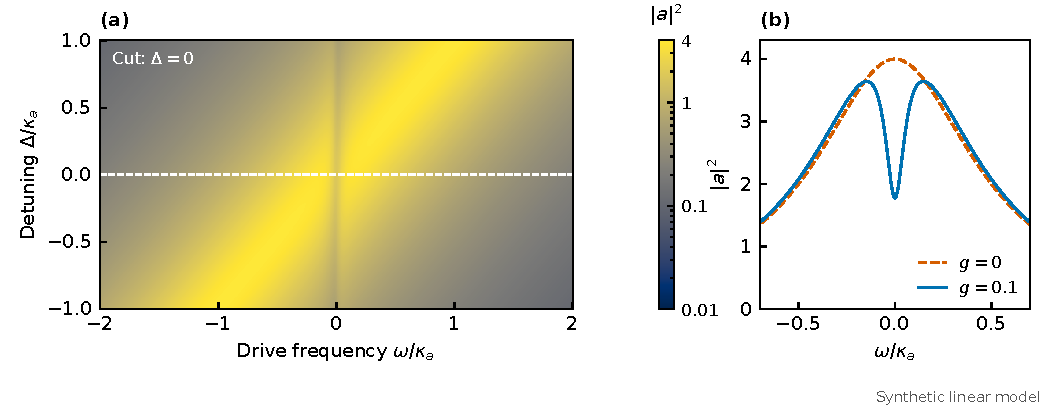
\includegraphics[width=\textwidth]{../mechanism-examples/response_map.pdf}
\caption{Synthetic response map and supporting spectrum. A cross-column float preserves the dominant-map hierarchy and readable axis labels. Numerical values are generated by the documented two-mode model, not inferred experimental data.}
\label{fig:response}
\end{figure*}

\textit{Interpretation and layout.---}The pole calculation identifies the available decay channels, while the response describes their excitation by a chosen drive. Establishing a manuscript's central mechanism would require connecting those observations to appropriate controls and to the closest prior work. This deliberately incomplete demonstration cannot replace that scientific comparison. Its short text also makes the influence of float placement especially visible: a wide figure may move to a later page despite appearing earlier in the source. In a real paper, organize the evidence and adjust the physical figure dimensions before attempting to force positions.

\textit{Conclusion.---}The model distinguishes a weak-coupling slow mode from the equal-damping regime through its actual eigenvalues. This supported distinction is the physical statement; the example's single-column and wide figures merely show two ways to allocate space to the corresponding evidence. The file is a layout demonstration, not a length-limit certification or an example of a fully developed introduction.
\end{document}
